\section{EAC}
\label{sec:eac results}

This section will present thorough results concerning several characteristics related to the EAC method.
These were the timings of the different parts, how the number of patterns and the different $K_{min}$ rules affected the sparsity of the co-association matrix, the typical number of associations per cluster in each rule, the growth of the number of associations with the different parameters, among others.
Two 2-dimensional 10 million pattern mixtures of 6 Gaussians were generated.
A variation of the number of dimensions has more interest in the performance characteristics of the production phase.
Since the production of the ensemble uses K-Means, detailed results can be found in section \ref{sec:parallel kmeans}.
One mixture has overlapping Gaussians and the other has not.
% The reasoning was that overlapping Gaussians might result in more associations per cluster.
The results contained in this section refer to the dataset with overlapping Gaussians, but the same overall patterns can be found in the other and the same conclusions can be drawn.

Different rules for computing the $K_{min}$, different co-association matrix formats and different approaches for the final clustering will be mentioned.
The different rules and their aliases are presented in Table \ref{tab:eac rules}.
The different formats for the co-association matrix are the \emph{full} (for fully allocated $n \times n$ matrix), \emph{full condensed} (for a fully allocated $\frac{n(n-1)}{2}$ array to build the upper triangular matrix), \emph{sparse complete} (for EAC CSR), \emph{sparse condensed const} (for EAC CSR building only the upper triangular matrix) and \emph{sparse condensed linear} (for EAC CSR condensed).
The different approaches for the final clustering are \emph{SLINK} \cite{Sibson1973}, \emph{SL-MST} (for using the Kruskal implementation in SciPy) and \emph{SL-MST-Disk} for the modified version that performs an external memory sort.

\begin{table}[h]
\centering
\caption{Different rules for computing $K_{min}$ and $K_{max}$. $n$ is the number of patterns and $sk$ is the number of patterns per cluster.}

\begin{tabular}{lcc}
\toprule
Rule &  $K_{min}$ &  $K_{max}$ \\
\midrule
\emph{sqrt}     & $\frac{\sqrt{n}}{2}$      & $\sqrt{n}$    \\
\emph{2sqrt}    & $\sqrt{n}$                & $2 \sqrt{n}$  \\
\emph{sk=sqrt2} & $sk = \frac{\sqrt{n}}{2}$ & $1.3 K_{min}$ \\
\emph{sk=300}   & $sk = 300$                & $1.3 K_{min}$ \\
\bottomrule
\end{tabular}

\label{tab:eac rules}
\end{table}

The experiment that generated the results of these section was set up as follows.
A large dataset was generated.
The dataset was sampled uniformly to produce a smaller dataset with the desired number of patterns.
A clustering ensemble was produced (production phase) for each of these smaller datasets and for each of the rules, using K-Means.
From each ensemble, co-association matrices of every applicable format were built (combination phase).
A matrix format was not applicable when the dataset complexity would make its correspondent co-association matrix too big to fit in main memory.
The final clustering (recovery phase) was also done for each of the matrix formats.
SLINK was used with fully allocated formats and the MST-based SL (SL-MST) and MST-based SL on external memory (SL-MST-disk) were executed with sparse matrices.
SL-MST was not executed if its space complexity was too big to fit in main memory.
Furthermore, the combination and recovery phases were repeated several times for smaller datasets for statistical relevant of the execution times, so as to make the influence of any background process less salient.
For big datasets, the execution times are big enough that the influence of background processes is negligible.

All results presented here originated from machine Bravo.

\subsection{Performance of production and combination phases}

The $K_{min}$ parameter, whose evolution is presented in Fig. \ref{fig:eac kmin evo}, influences several other EAC properties.
Rules \emph{sqrt}, \emph{2sqrt} and \emph{sk=sqrt2} never intersect with the increase if the number of patterns, but rule $sk=300$ intersects the others, finishing with the highest $K_{min}$.

\begin{figure}[hbt!]
    \centering
    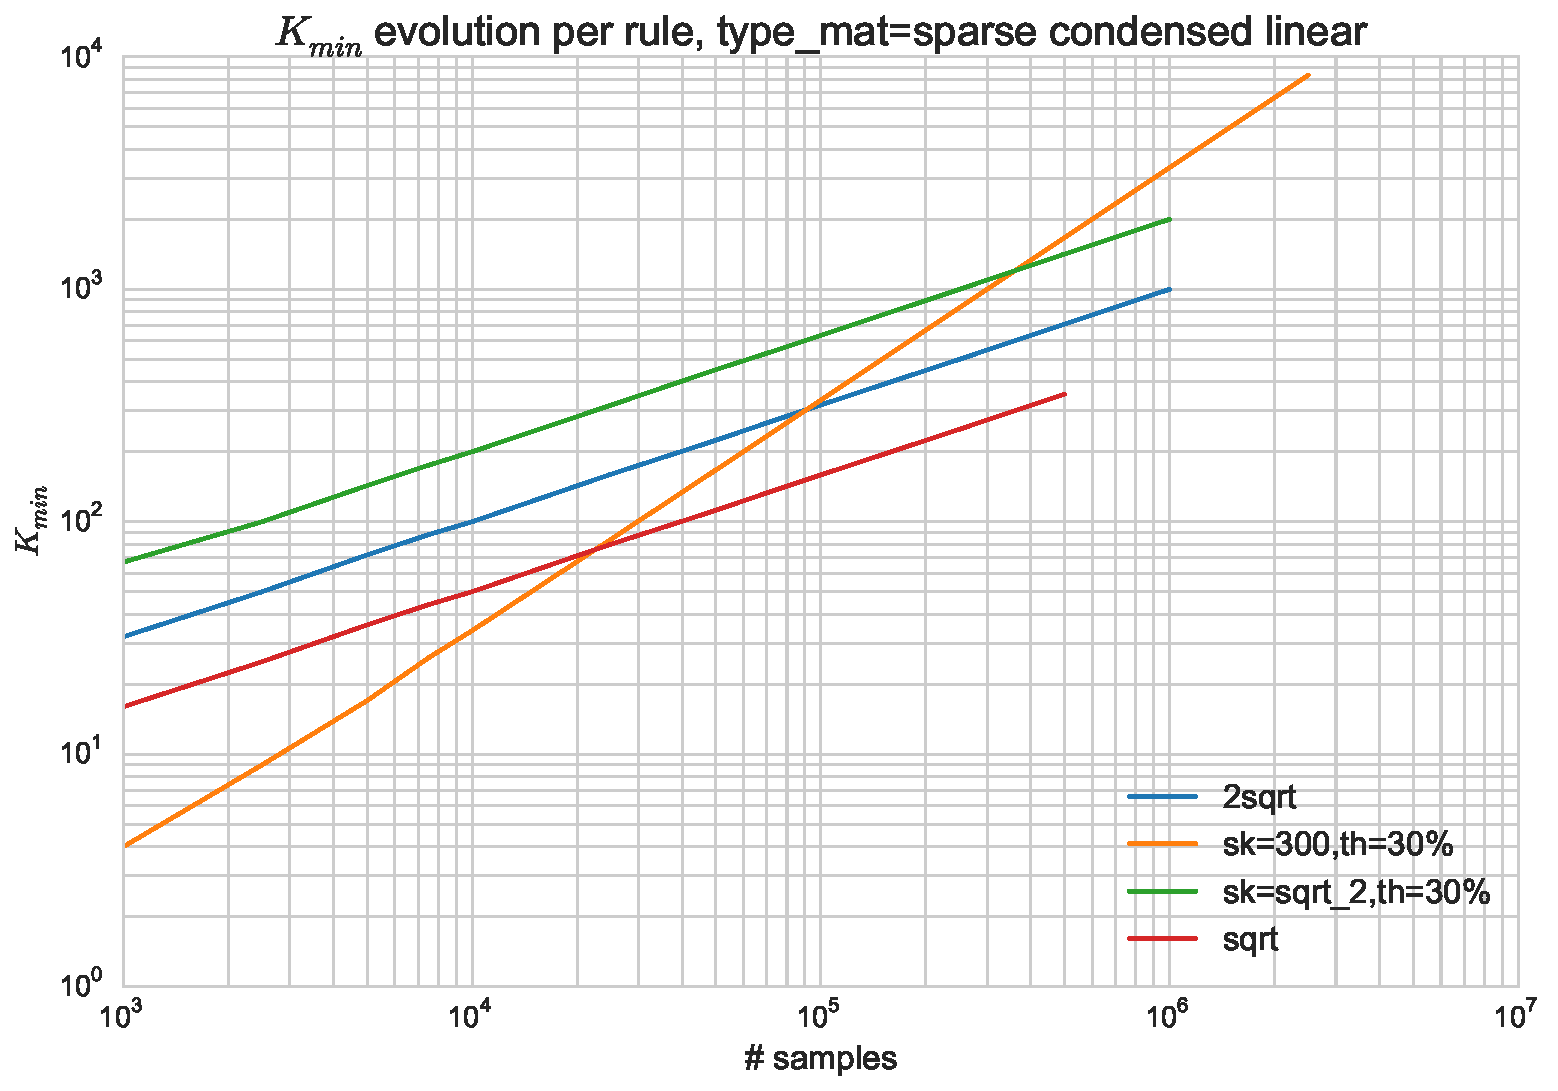
\includegraphics[width=0.6\textwidth]{{{results/eac/kmin_evolution}}}
    \caption{Evolution of $K_{min}$ with cardinality for different rules.}
    \label{fig:eac kmin evo}
\end{figure}

The execution times for the production and combination phase can be observed in Figures \ref{fig:eac ensemble times}, \ref{fig:eac build rules} and \ref{fig:eac build matrices}, which allow the comparison between the different rules and the different matrix formats, respectively.
To avoid redundancy, only one matrix format is depicted to compare the execution times for the different rules and only one rule to compare the matrix formats.
The results of the other cases follow the same pattern.
Observing Fig. \ref{fig:eac build rules}, one can see the tendency of the evolution of$K_{min}$ in the production execution time associated with the $sk=300$ rule and the inverse in the combination time.
A higher $K_{min}$ means more centroids for K-Means to compute, so it is not surprising that the execution time for computing the ensemble increases as $K_{min}$ increases.
On the other hand, a higher $K_{min}$ translates in more condensed clusters and less associations per pattern.
With less associations, the computation time for building the co-association matrix naturally decreases.

\begin{figure}[hbt!]
    \centering
    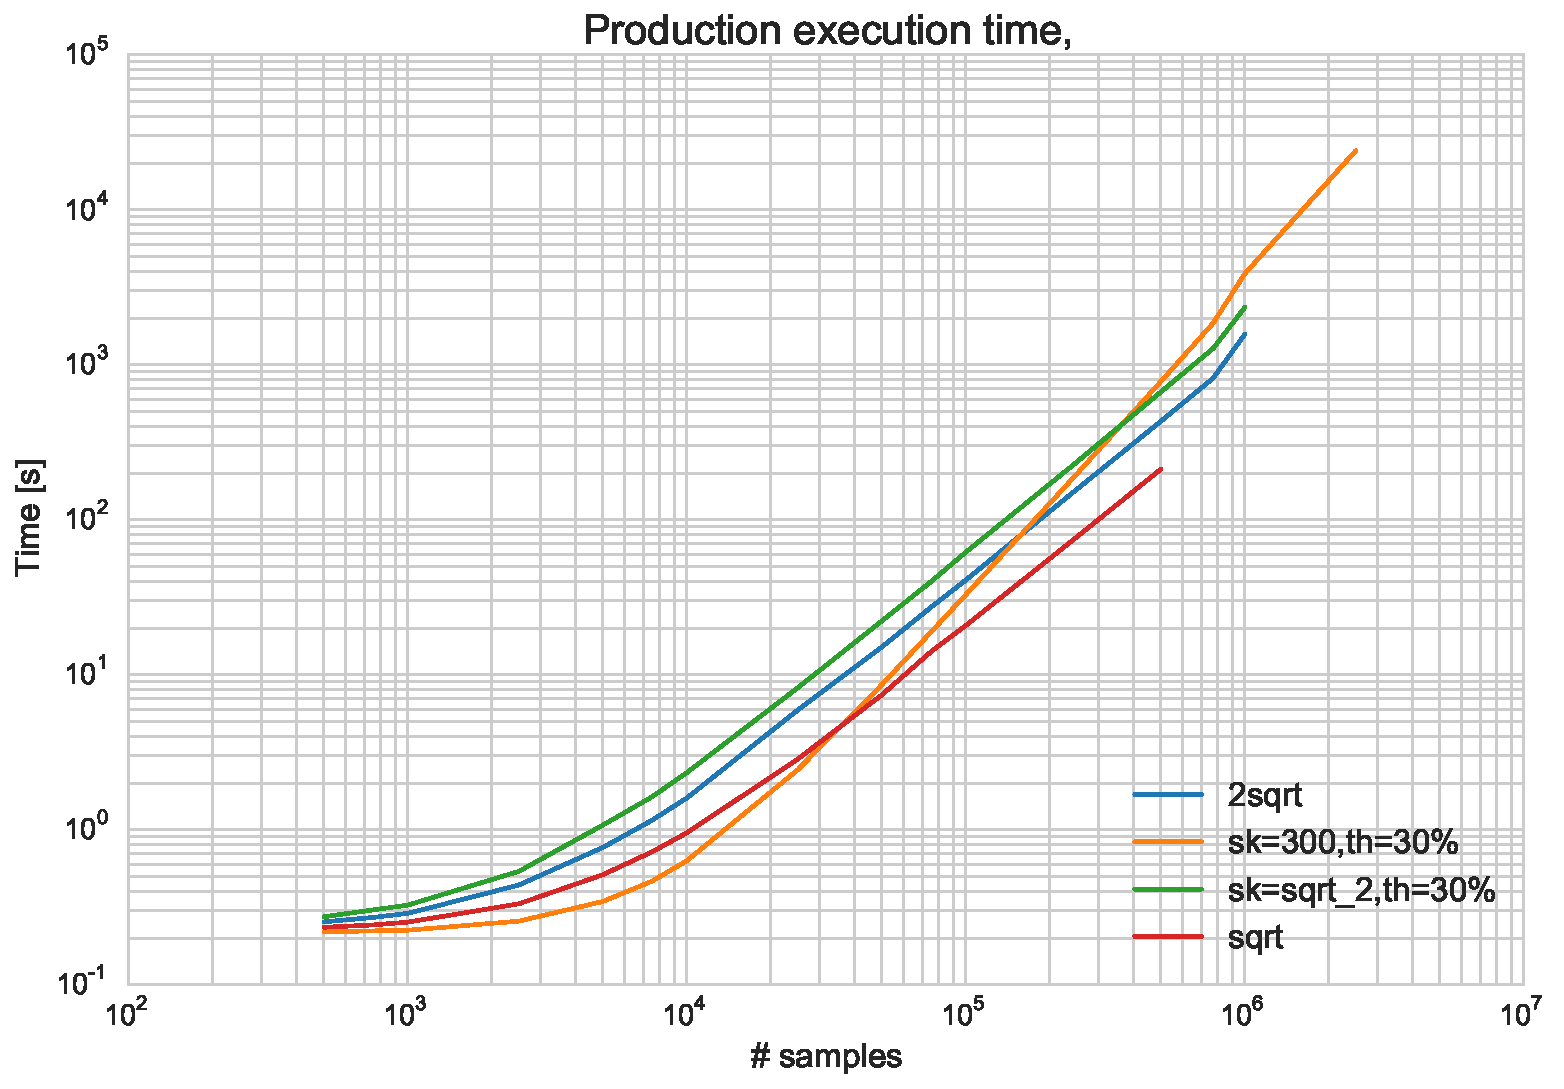
\includegraphics[width=0.6\textwidth]{{{results/eac/ensemble_time}}}
    \caption{Execution time for the production of the clustering ensemble.}
    \label{fig:eac ensemble times}
\end{figure}

\begin{figure}[hbt!]
    \centering
    \includegraphics[width=0.6\textwidth]{{{results/eac/build_time/sparse_condensed_linear}}}
    \caption{Execution time for building the co-association matrix from ensemble with different rules.}
    \label{fig:eac build rules}
\end{figure}

In a previous section, the execution times for the combination phase had already been briefly presented when comparing different sparse formats.
Fig. \ref{fig:eac build matrices} shows the execution times on a longitudinal study for optimized matrix formats.
It is clear that the sparse formats are significantly slower than the fully allocated ones, specially for smaller datasets.
The \emph{full condensed} format usually takes close to half the time than the \emph{full} format, which is natural given that it performs half the operations.
Idem for the \emph{sparse condensed} formats compared to the \emph{sparse complete}.
The big discrepancy between the sparse and full formats is due to the fact that the former needs to do a binary search at each association update and needs to keep the internal sparse data structure sorted.


\begin{figure}[hbt!]
    \centering
    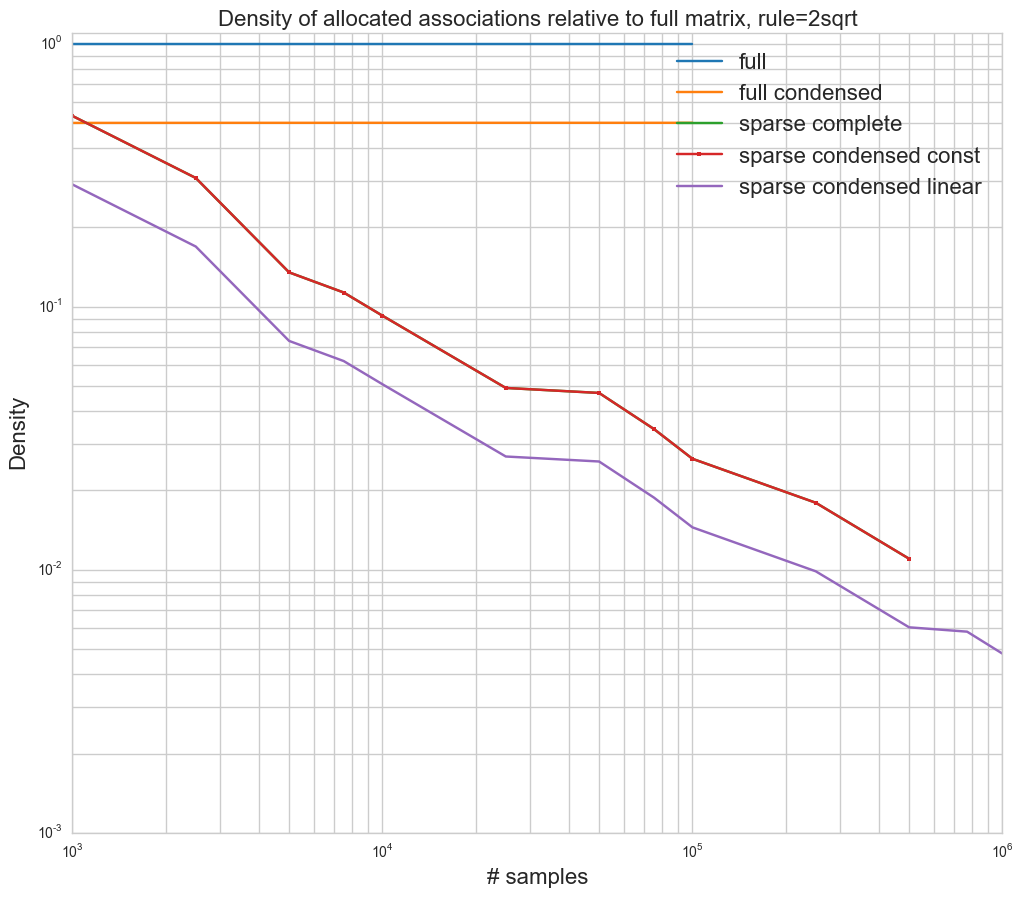
\includegraphics[width=0.6\textwidth]{{{results/eac/build_time/2sqrt}}}
    \caption{Execution time for building the co-association matrix with different matrix formats.}
    \label{fig:eac build matrices}
\end{figure}

\subsection{Performance comparison between SLINK, SL-MST and SL-MST-Disk}

The clustering times of the different methods of SL discussed previously (SLINK, SL-MST and SL-MST-Disk) are presented in Figures \ref{fig:eac sl}, \ref{fig:eac slink} and \ref{fig:eac sl-mst}.
The SL-MST-Disk method is significantly slower than any of the other methods.
This is expected, since it uses the hard drive which has very slow access times compared to main memory.
SL-MST is faster than SLINK, since it processes zero associations while SL-MST takes advantage of a graph representation and only processes the non-zero associations.
In resemblance to what happened with combination times, the condensed variants take roughly half the time has their complete counterparts.
This is expected, since SL-MST and SL-MST-Disk over condensed co-association matrices only process half the number of associations.
SLINK takes roughly the same time for every rule, which means $K_{min}$ has no influence, since SLINK processes the entire co-association matrix and $K_{min}$ only influences the number of non-zero associations.
The same rationale can be applied to SL-MST, where different rules can have significant influence over execution time, since they change the total number of associations.
As with the combination phase, the execution time referent to the \emph{sk=300} rule started with the greatest time and decreased with an increase in cardinality until it was the fastest.

\begin{figure}[hbt!]
    \centering
    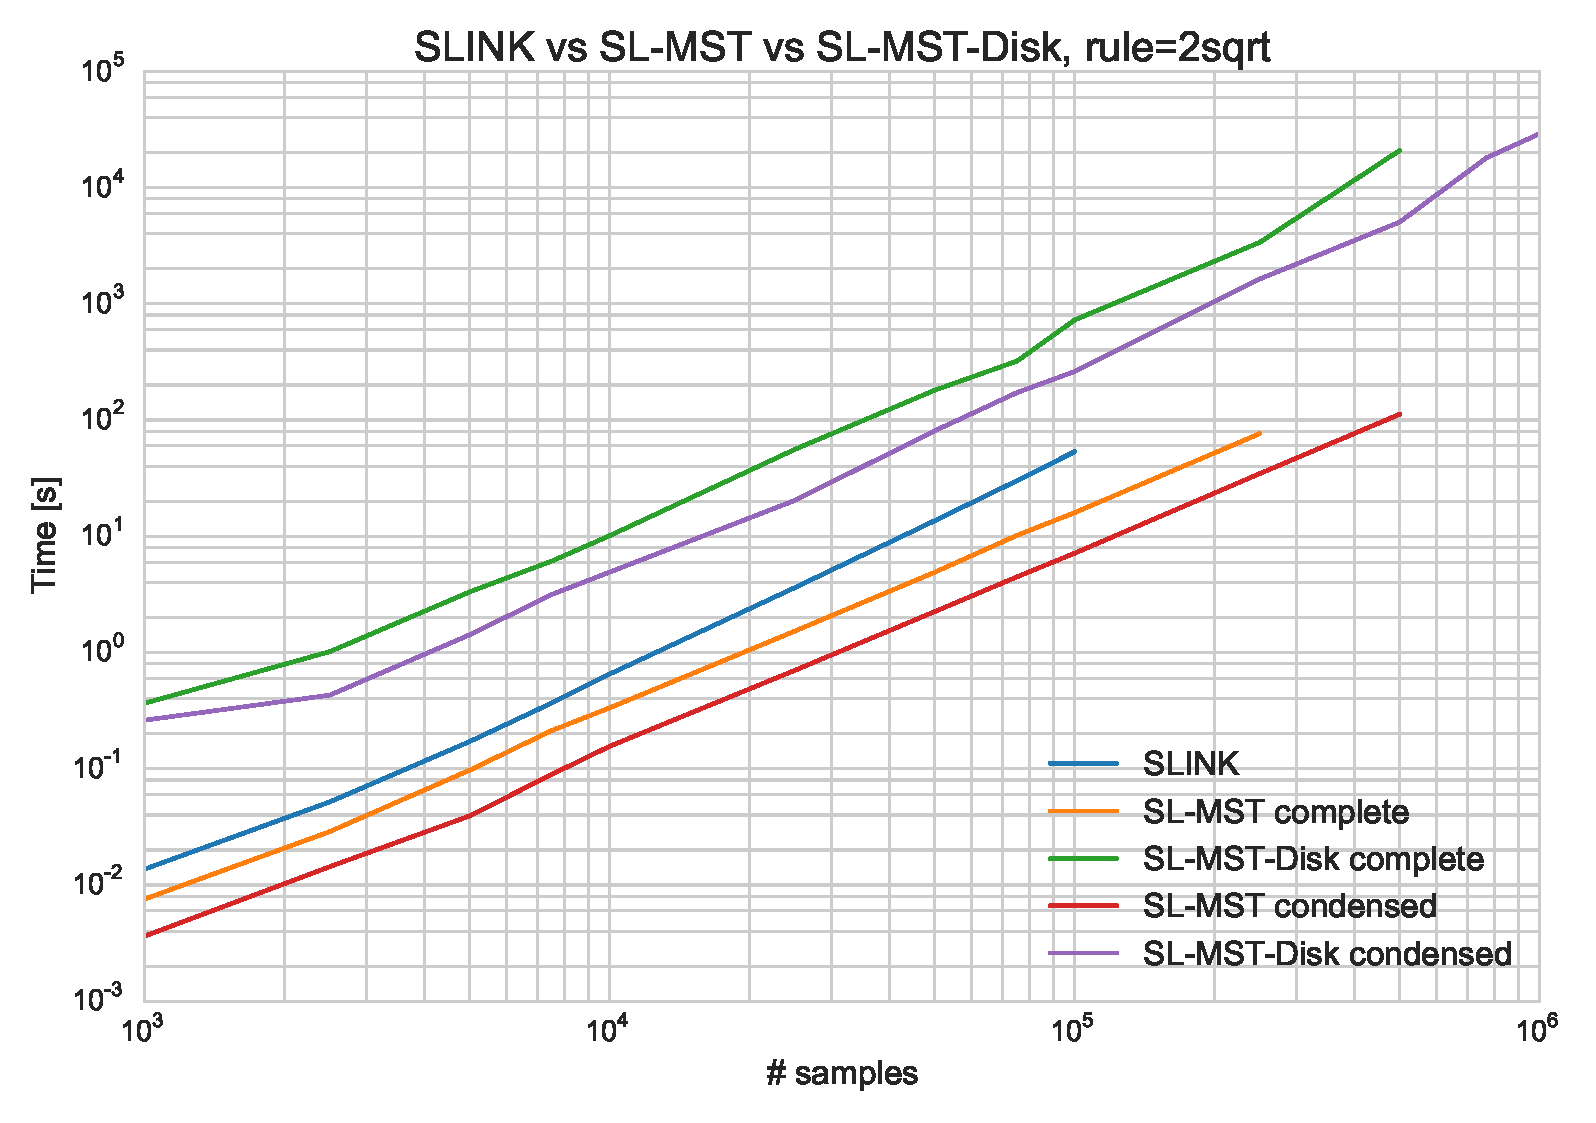
\includegraphics[width=0.6\textwidth]{{{results/eac/sl_time/slink_vs_sl-mst}}}
    \caption{Comparison between the execution times of the three methods of SL. SLINK runs over fully allocated condensed matrix while SL-MST and SL-MST-Disk run over the condensed and complete sparse matrices.}
    \label{fig:eac sl}
\end{figure}

\begin{figure}[hbt!]
    \centering
    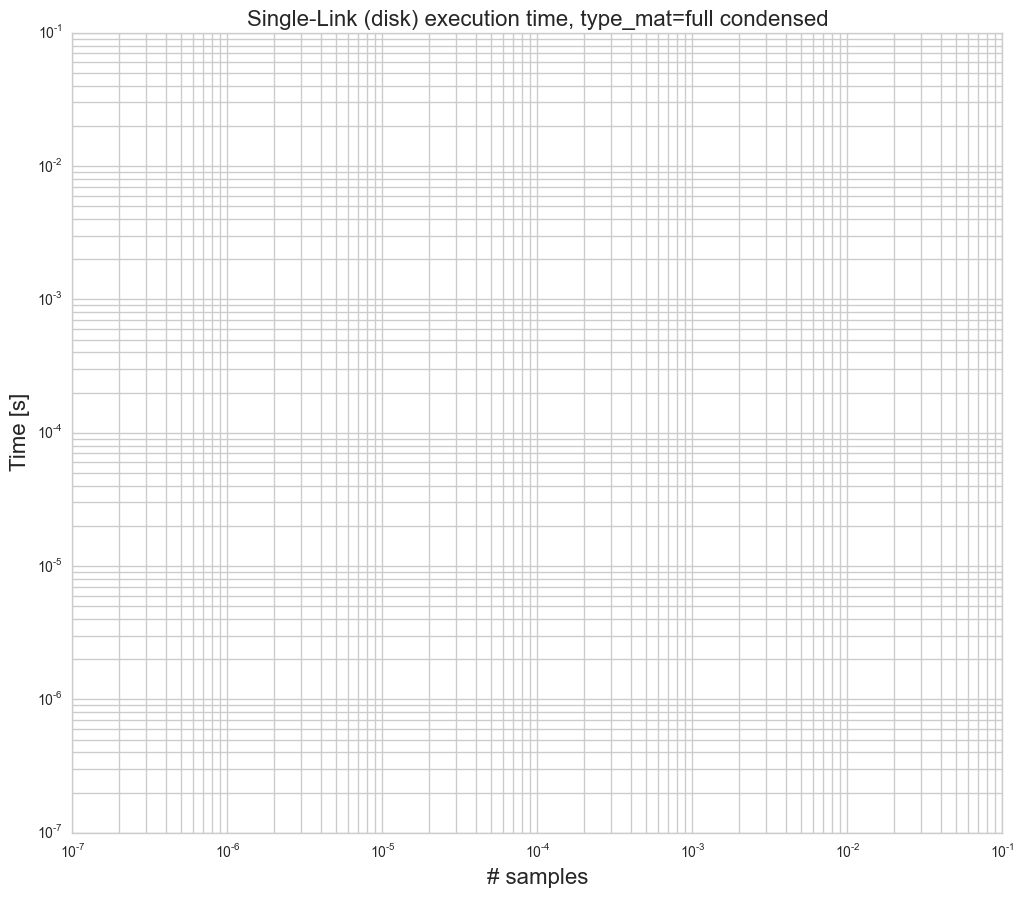
\includegraphics[width=0.6\textwidth]{{{results/eac/sl_mem_time/full_condensed}}}
    \caption{Comparison between the execution times of SLINK to different rules.}
    \label{fig:eac slink}
\end{figure}

\begin{figure}[hbt!]
    \centering
    \includegraphics[width=0.66\textwidth]{{{results/eac/sl_mem_time/sparse_condensed_linear}}}
    \caption{Comparison between the execution times of SL-MST for different rules.}
    \label{fig:eac sl-mst}
\end{figure}

\subsection{Performance of all phases combined}

The execution times of all phases combined are presented in Figures \ref{fig:eac total mem} and \ref{fig:eac total disk}.
The results are presented for the \emph{sparse condensed linear} format but the remaining results follow the same tendency.
It is interesting to note that, when using the SL-MST method in the recovery phase, the execution time for three of the rules do not differ much for large datasets.
This is due to a sort of balancing between a slowing down of the production phase and a speeding up of the combination and recovery phases as the $K_{min}$ increases at a higher rate for $sk=300$ than for other rules.
This is not observed for the $sqrt$ rule as $K_{min}$ is always low enough that the total time is always dominated by the combination and recovery phases.
The same does not happen when using the SL-MST-Disk method, as the total time is completely dominated by the recovery phase.
This is clear, since the results in Fig. \ref{fig:eac total disk} follow a pattern similar to that presented in Fig. \ref{fig:eac sl-mst}.


\begin{figure}[hbt!]
    \centering
    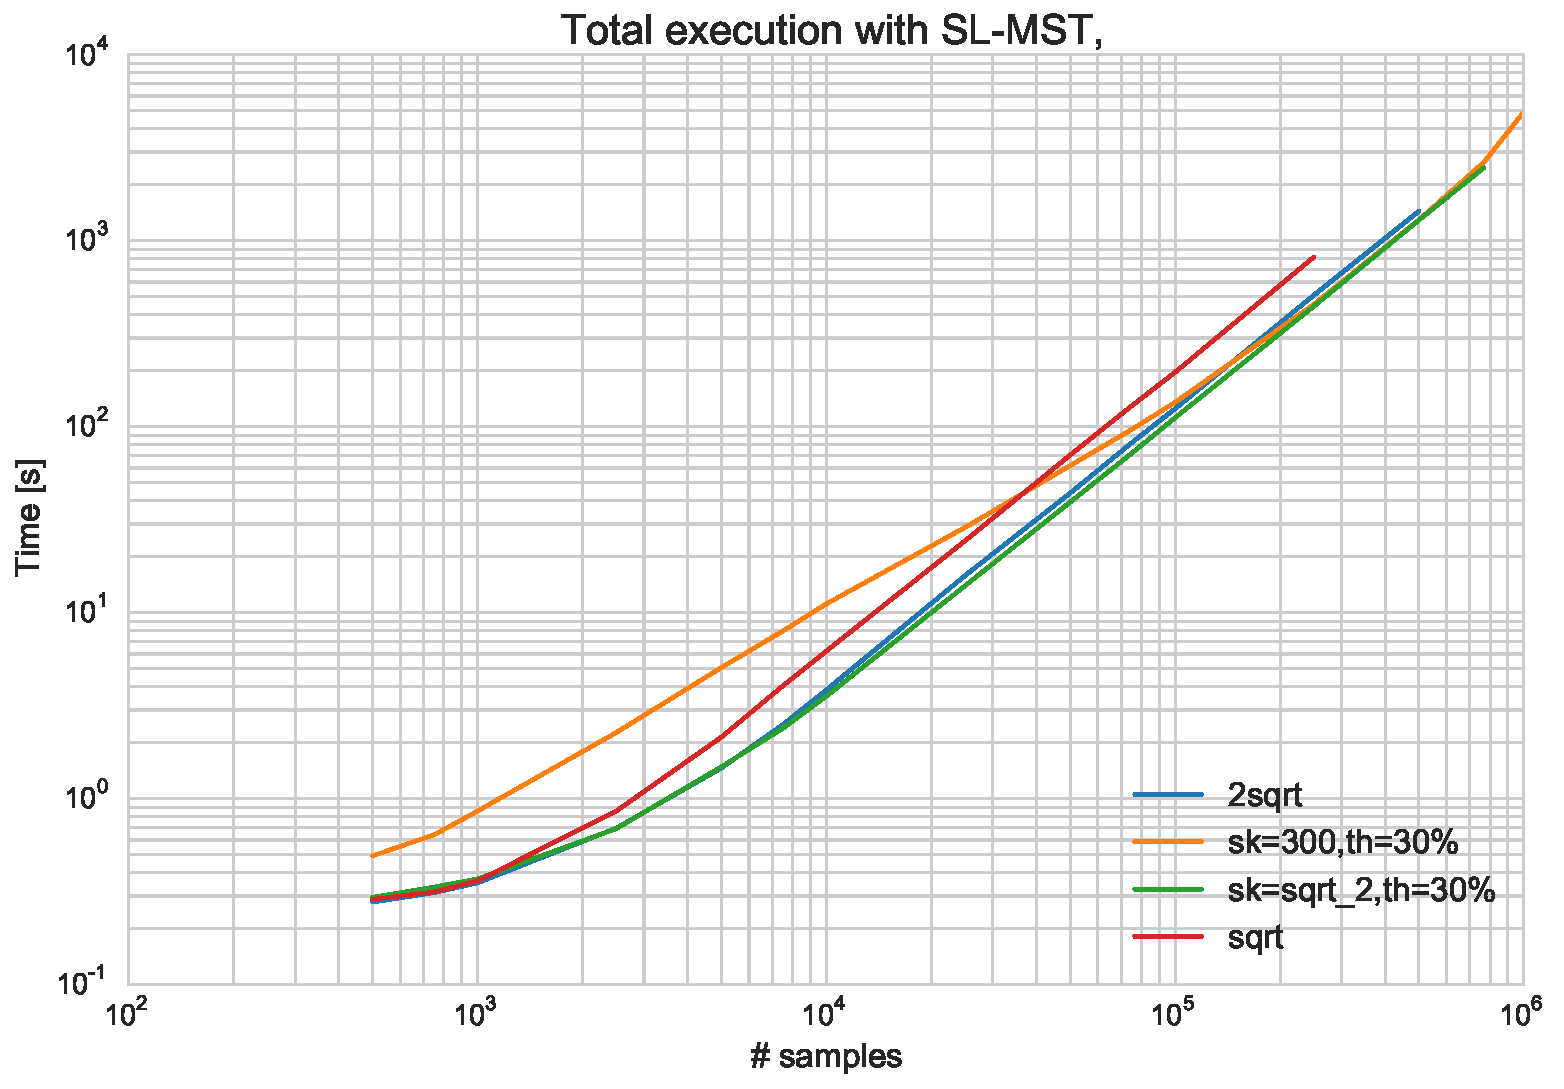
\includegraphics[width=0.6\textwidth]{{{results/eac/total_time_sl-mst}}}
    \caption{Execution times for all phases combined, using SL-MST in the recovery phase.}
    \label{fig:eac total mem}
\end{figure}

\begin{figure}[hbt!]
    \centering
    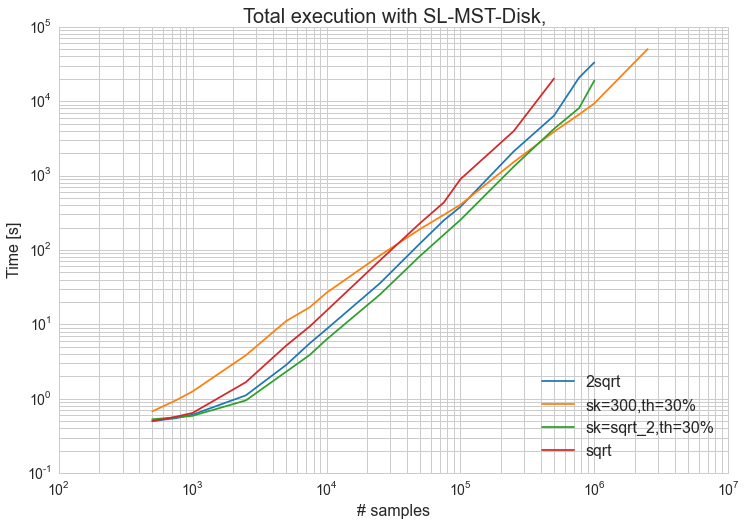
\includegraphics[width=0.66\textwidth]{{{results/eac/total_time_sl-mst-disk}}}
    \caption{Execution times for all phases combined, using SL-MST-Disk in the recovery phase.}
    \label{fig:eac total disk}
\end{figure}


\subsection{Analysis of the number of associations}

The sparse nature of EAC has been pointed out before and is clearer in Fig. \ref{fig:eac assoc density}.
This figure shows the association density, i.e. number of associations relative to the $n^2$ possible associations in a full matrix.
The \emph{full condensed} format maintains a density of roughly $50\%$ and the density of \emph{sparse complete} is two times that of the \emph{sparse condensed} formats.
The overall tendency is for the density to decrease as the number of patterns of the dataset increases.
This is to be expected since the \emph{full} matrix grows quadratically.
Besides, it would be expected that the same associations would be grouped together more frequently in partitions and simply make previous connections stronger instead of creating new ones.
Results presented in Fig. \ref{fig:eac assocs per pattern}, which presents the number of associations per pattern, suggest that but it is only clear for the $sk=300$ rule.
The number of associations per pattern increases with the number of patterns of the dataset, with the notable exception of the \emph{sk=300} rule which increases until it reaches a certain limit and then stabilizes.
This is explained by the fact that this rule is based on setting a maximum constant number ($300$) of patterns in any given cluster, while in the other rules this number increases with the number of patterns.
The number of associations per pattern is not $300$ for the $sk=300$ rule because a pattern will be clustered with different neighbors in different partitions.
Still, the number of neighbors doesn't change enough that the number of associations per pattern increases boundlessly.
In fact, Fig. \ref{fig:eac assocs per pattern} suggests that the number of associations per pattern is around 3 times the upper bound on the number of patterns per cluster (strictly related to $K_{min}$).
This is clearer for $sk=300$, but if one would trace the the number of patterns divided by $K_{min}$ for each rule, a similar tendency would manifest.
\citet{Lourenco2010} reported that, on average, \"the overall contribution of the clustering ensemble (including unbalanced clusters) duplicates the co-associations produced in a single balanced clustering with Kmin clusters\".
The spectrum of datasets evaluated regarding number of patterns was smaller than that evaluated in the present work.
The present results suggest a slightly higher value.
So, the decrease in density is more related with the quadratic growth of the \emph{full} matrix in contrast with a linear growth of the number of associations.

\begin{figure}[hbt!]
    \centering
    \includegraphics[width=0.6\textwidth]{{{results/eac/assoc_density/sparse_condensed_linear}}}
    \caption{Density of associations relative to the full co-association matrix, which hold $n^2$ associations.}
    \label{fig:eac assoc density}
\end{figure}

\begin{figure}[hbt!]
    \centering
    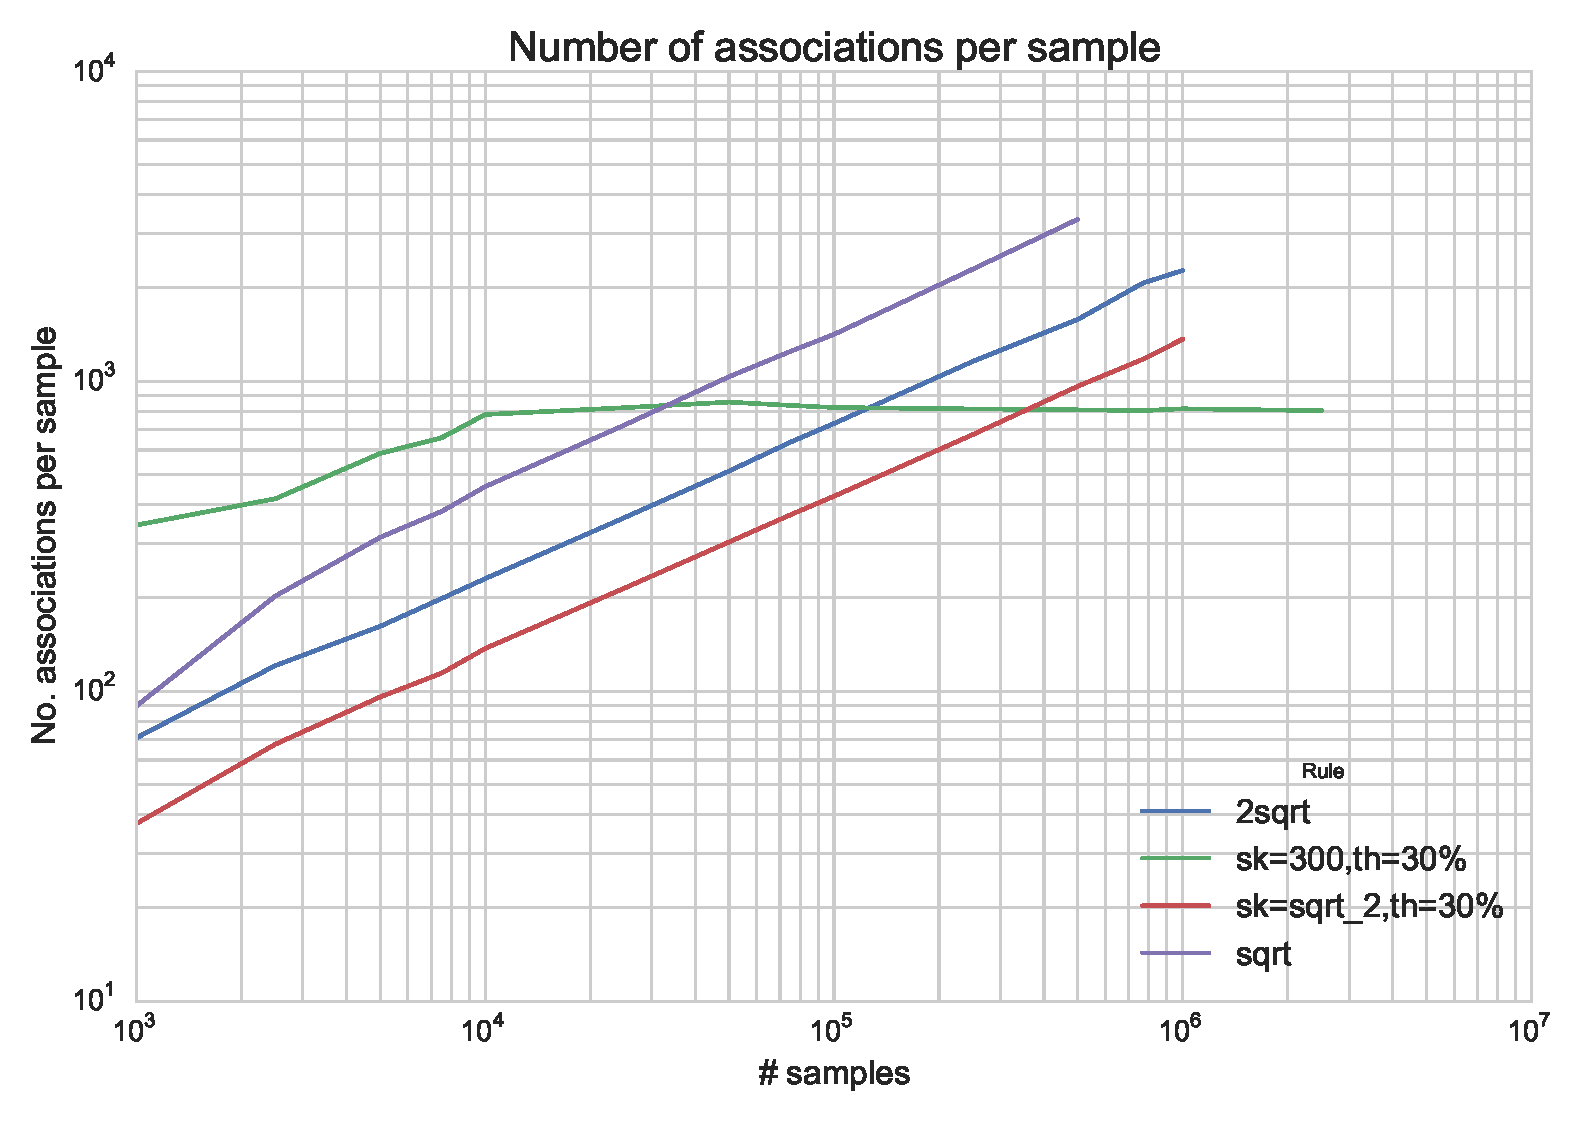
\includegraphics[width=0.6\textwidth]{{{results/eac/assocs_per_sample}}}
    \caption{Evolution of the total number of associations divided by the number of patterns according to the different rules.}
    \label{fig:eac assocs per pattern}
\end{figure}

Predicting the number of associations before building the co-association matrix is useful for coming up with combination schemes that are both memory and speed efficient.
It was stated before that the biggest cluster size in any partition of the ensemble is a good parameter for this end.
Fig. \ref{fig:eac max assocs per bgs} presents the relationship between the biggest cluster size and the maximum number of associations of any pattern.
These ratio increases with the number of patterns in the beginning, but as the number of patterns increases it never goes over 3.

\begin{figure}[hbt!]
    \centering
    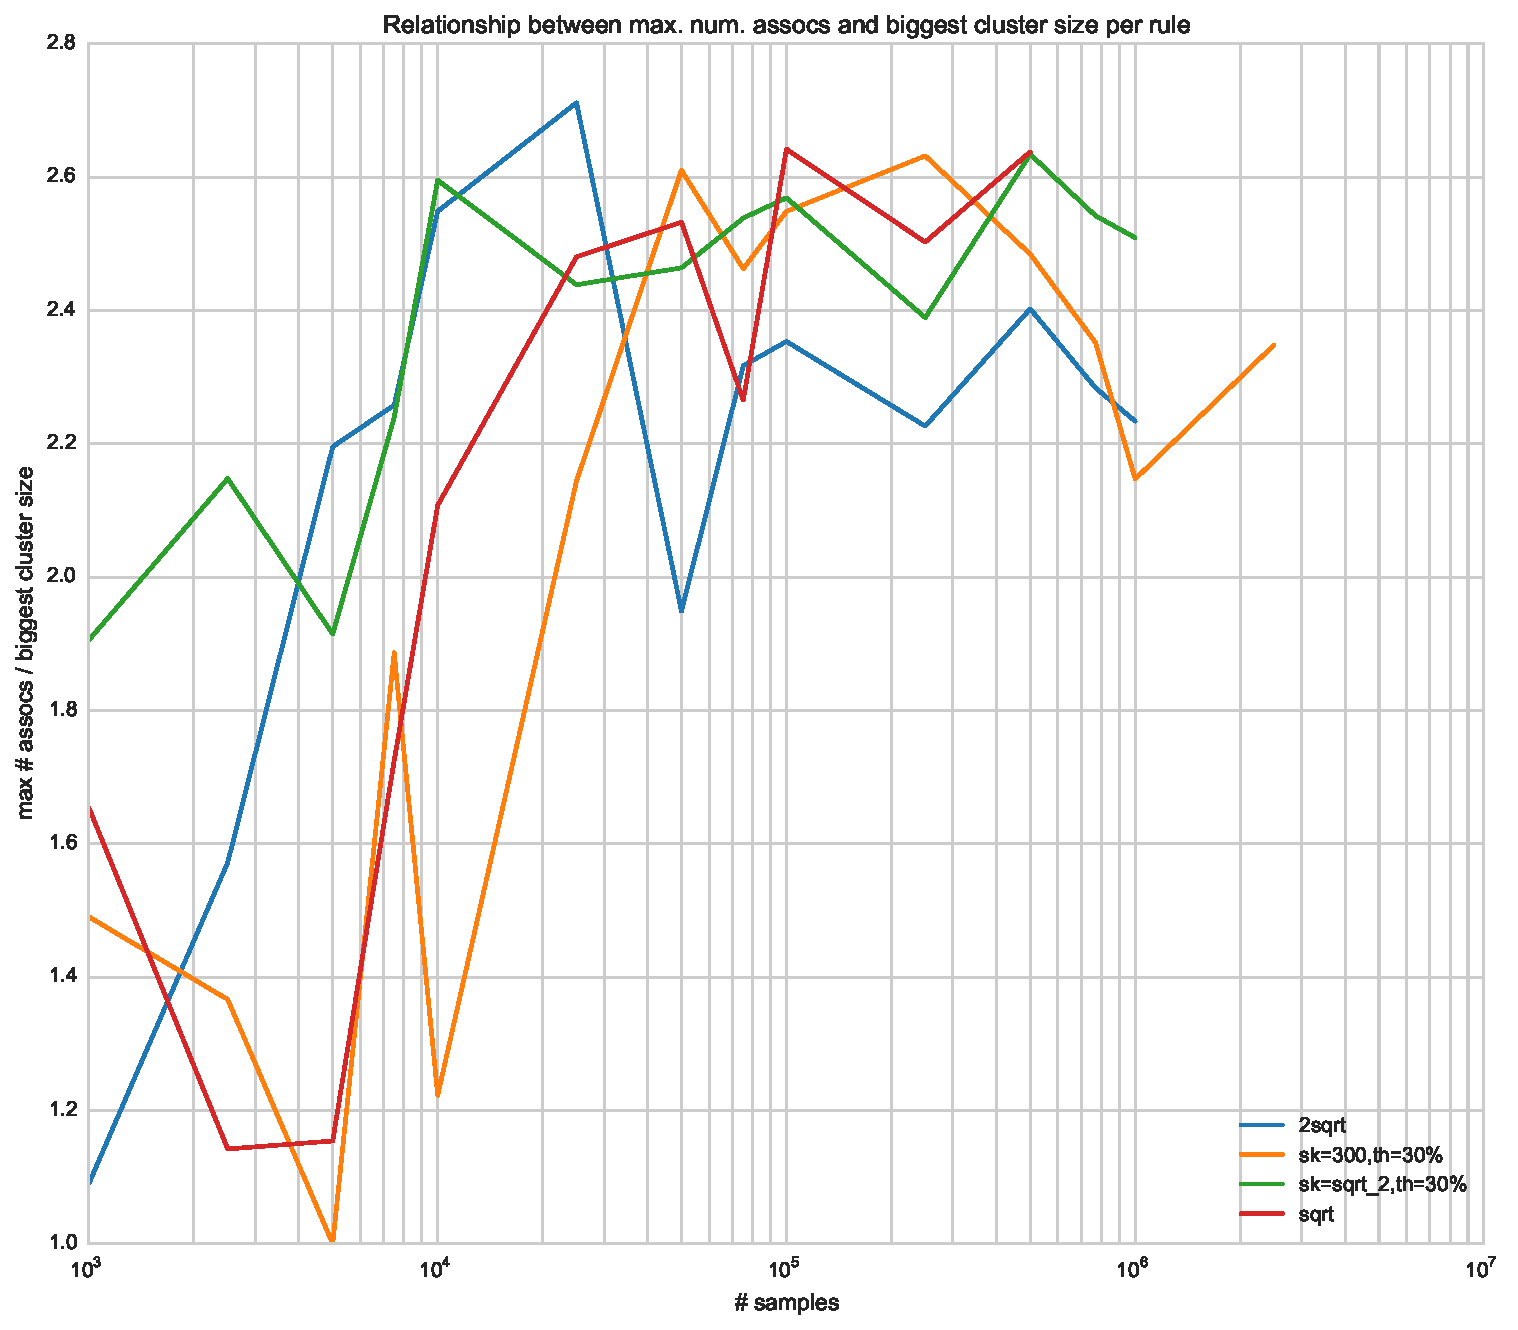
\includegraphics[width=0.6\textwidth]{{{results/eac/max_assoc_bgs}}}
    \caption{Maximum number of associations of any pattern divided by the number of patterns in the biggest cluster of the ensemble.}
    \label{fig:eac max assocs per bgs}
\end{figure}

However, the number of features of the used datasets is rather reduced.
It might be the case that this ratio would increase with the number of features, since there would be more degrees where the clusters might include other neighbors.
With this in mind, further studies ranging a wider spectrum of datasets should yield more enlightening conclusions or reinforce those presented here.

\subsection{Space complexity}

The previous section analyzed results related to the number of associations.
This is related to the space complexity of the different matrix formats, but does not present an accurate depiction of their complexity, mainly due to the data structures supporting the sparse formats.
The true space complexity of the formats can be observed in Figures \ref{fig:eac allocated density} and \ref{fig:eac mem density}.

As explained previously, the allocated space for the space formats is based on a prediction that uses the biggest cluster size of the ensemble.
This allocated space is usually more than what is necessary to store the total number of associations.
Furthermore, the CSR sparse format, on which the EAC CSR strategy is based, requires an array of the same size of the predicted number of associations.
This overhead may in fact make the sparse format pre-allocate more associations than actually are possible for some rules, as can be seen in Fig. \ref{fig:eac allocated density}.
Still, the allocated number of associations becomes a very small fraction compared to the \emph{full} matrix as the dataset complexity increases, which is typical case for using a sparse format.

\begin{figure}[hbt!]
    \centering
    \includegraphics[width=0.6\textwidth]{{{results/eac/allocated_density/sk=300}}}
    \caption{Allocated number of associations relative to the full $n^2$ matrix.}
    \label{fig:eac allocated density}
\end{figure}

The actual memory used, presented in Fig. \ref{fig:eac mem density}, follows roughly the same pattern.
Here, the data types used play a big role in the amount of memory that is required.
Each association was stored in a single byte, since the number of partitions was less than 255, as is usually the case.
This means that the memory used by the fully allocated formats is $n^2$ and $\frac{n(n-1)}{2}$ Bytes for the fully allocated complete and condensed formats, respectively.
In the sparse formats, the values of the associations were stored in an array of unsigned integers of 1 Byte.
However, an array of integers of 4 Bytes of the same size existed to keep track of the destination pattern each association belongs to.
Besides, one other array of integers of 8 Bytes is kept but it is negligible compared to the other two arrays.
The impact of the data types can be seen for smaller datasets where the total memory used is actually significantly higher than that of the \emph{full} matrix.
It should be noted that this discrepancy is not as high for other rules as for $sk=300$.
Still, the sparse formats, and in particular the condensed sparse format, is preferred since the memory used for large datasets is a small fraction of would be necessary if using any of the fully allocated formats.
The data types used depend on the problem at hand, since a user may choose to use a large ensemble or have a very large 

\begin{figure}[hbt!]
    \centering
    \includegraphics[width=0.6\textwidth]{{{results/eac/mem_density/sk=300}}}
    \caption{Memory used relative to the full $n^2$ matrix.}
    \label{fig:eac mem density}
\end{figure}

\subsection{Accuracy}

Finally, the accuracy of each solution was measured and is presented in Fig. \ref{fig:eac accuracy}.
The number of clusters of the final solutions was determined by the lifetime method.
The accuracy was the same for all rules and for all matrix formats in each dataset, except in the beginning were the $sk=300$ produces bad results due to the ensemble having partitions with a number of clusters inferior to the real number of clusters.
Still, the $sk=300$ rule is the one presented because it spans a wider spectrum of datasets.
When two classes are overlapping, the lifetime method typically interprets them as being the same class.
In the beginning, there are only two overlapping Gaussians, explaining the accuracy of roughly $84\%$.
As more patterns are added to the datasets, the accuracy lowers to around $66\%$, since now 4 classes are overlapped in pairs.
There are two lows in accuracy around the $50\%$.
The first is due to a "bridge" between two classes by a couple of patterns that are not present in the surrounding datasets duo to sampling.
The last is duo to the same reason, since now more patterns are included in the dataset.

\begin{figure}[hbt!]
    \centering
    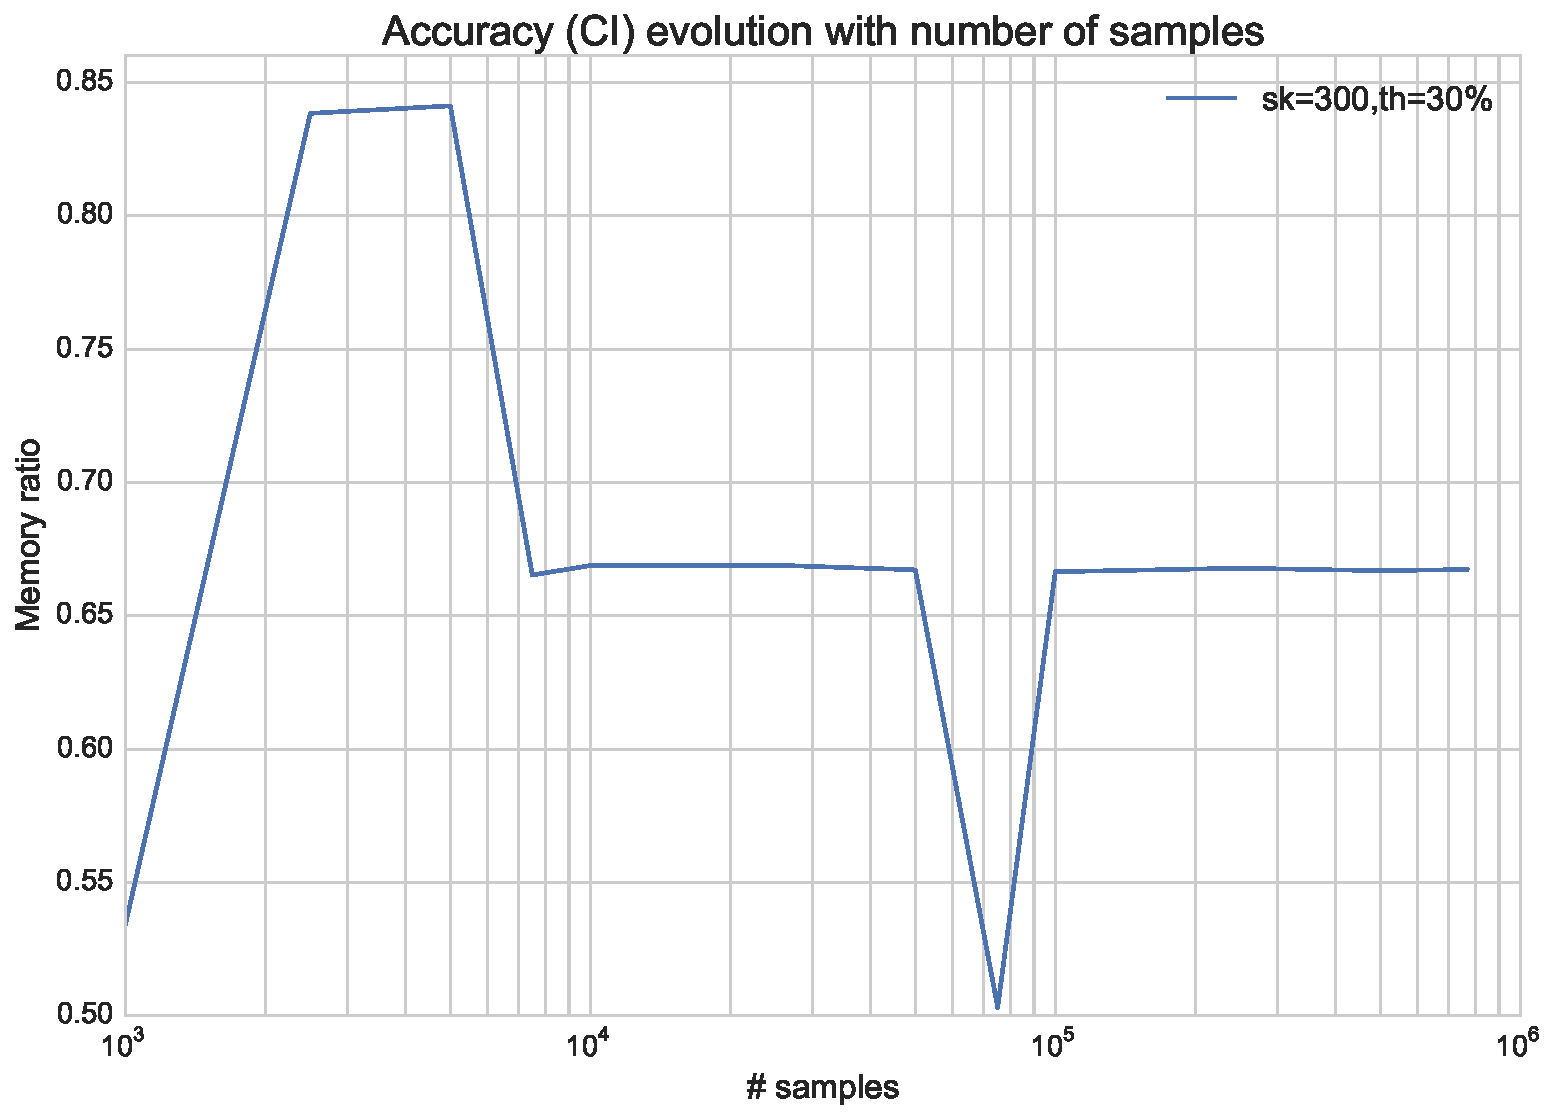
\includegraphics[width=0.6\textwidth]{{{results/eac/accuracy}}}
    \caption{Accuracy of the final clusterings as measured with the Consistency Index.}
    \label{fig:eac accuracy}
\end{figure}

\section{Performance on real world datasets}

The proposed EAC method was tested on real world datasets.
Large real world datasets appropriate for clustering were hard to find freely available.
The datasets used are aimed at other Machine Learning analysis, such as classification or regression.
For this reason, the presented results are focused on performance.
Table \ref{tab:eac big real} presents execution times for different phases of EAC on several real world datasets.
The ensemble size was of 30, the combination phase used sparse condensed matrices and the \emph{sk=300} rule and the recovery phase was done with SL based on main memory.
No comparison is possible with the original implementation, since computation would not be possible.
In most datasets the production phase took the longest.
The reason for this is that clusters in the ensemble were small which led to fewer associations and, thus, more time spent in the production phase than in the others.
Furthermore, the recovery phase was fast because SL was based on main memory.
Although high, the computation times are acceptable for the processing of large datasets with a robust algorithm such as EAC in a typical workstation.

\begin{table}[h]
\centering
\caption{Execution times for real-world large datasets. P and F refer to the number of patterns and features. P, C and R times refer to the production, combination and recovery times.}

\begin{tabular}{llrrrrr}
\toprule
dataset alias                                 &  \# P               &  \# F               &  P time [s]  &  C time [s] &  R time [s] \\
\midrule
PHYACT 1 \cite{Lichman:2013}                  &              441568 &                  30 &      2158.69 &      123.85 &      19.76 \\
PHYACT 2 \cite{Lichman:2013}                  &              359170 &                  30 &      1477.34 &       98.86 &      15.79 \\
esopH \cite{yuk13oro}                         &              136127 &                   2 &        17.94 &       35.15 &       3.95 \\
diabetes \cite{strack2014impact,Lichman:2013} &              101766 &                  41 &       188.56 &       36.79 &       5.07 \\
\bottomrule
\end{tabular}


\label{tab:eac big real}
\end{table}